\section{Returning Results to the Frontend}
\label{sec:visitor}

As mentioned in \cref{sec:overview}, every command implementing the
\texttt{``IReplCommand''} interface should return an instance of a class
implementing the \texttt{``IResult''} interface. It is up to the implementing
frontend to determine how to display the result. Since commands can fail or
result in an exception (see \cref{sec:function-comp}), it is not always clear
what kind of \texttt{``IResult''} the command will return.

To illustrate this, it is certainly possible that a user tries to evaluate an
input that passes the parsing step but fails with an exception at the analyze
step (see \cref{fig:unit-flow}).  The expected result is an
\texttt{``EvaluateResult''}, but because an exception was thrown the
corresponding wrapped \texttt{``AnalyzeUnit''} cannot be created.

The visitor pattern has been adopted to solve this problem. As can be seen in
\cref{fig:uml-visitor}, every \texttt{``IResult''} can be ``visited'' by classes
implementing the \texttt{``IResultVisitor''} interface. Any class implementing
this interface can then decide per result type how to display the returned
information. Since all commands can always return a result with the original
exception or the failed \texttt{``ISpoofaxResult''}, the frontend is always
provided with error messages as well as the results of earlier processing steps.

\begin{figure}[h]
  \centering
  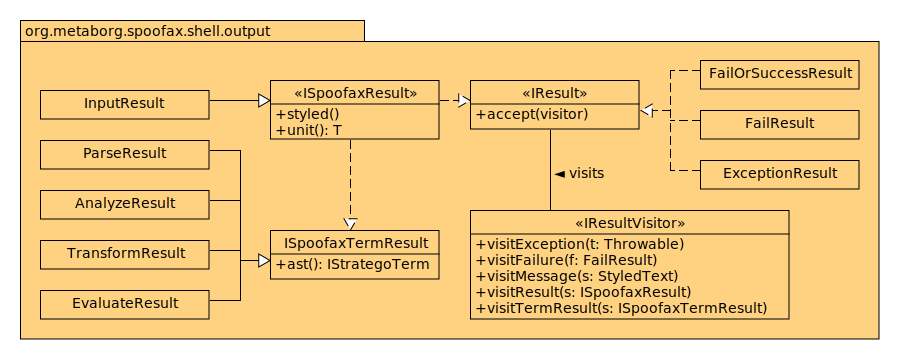
\includegraphics[width=0.8\textwidth]{uml-visitor}
  \caption{UML of the various concrete results and the result visitor.}
  \label{fig:uml-visitor}
\end{figure}

The frontend has the responsibility to decide how to present the returned data
to the user, resulting in a lot of flexibility. This flexibility is not always
required. It is not necessary, for example, for a text-based console REPL,
although it can be used to easily highlight errors or print stack traces. When
integrating the REPL in multithreaded GUI toolkits, however, this flexibility is
very useful.
